\def\true{true}
\let\fplncs\true
\documentclass{llncs}
\usepackage{amsmath}
\usepackage{amssymb}
\usepackage{graphicx}
\usepackage[utf8]{inputenc}
\usepackage{mathpartir}
\usepackage{moreverb}
\usepackage{xspace}
\usepackage{mymacros}
\usepackage{mytheorems}
\usepackage{fppdf}
%\usepackage[bookmarks=false,colorlinks=true,linkcolor=blue,citecolor=blue,urlcolor=blue]{hyperref}
\usepackage{mystmaryrd}
% EBNF syntax.

\let\nt\textit % Nonterminal.
\newcommand{\is}{& ${} ::= {}$ &}
\newcommand{\optional}[1]{$[\,\text{#1}\,]$} % Option.
\newcommand{\seplist}[2]{#2#1${}\ldots{}$#1#2}
\newcommand{\sepspacelist}[1]{\seplist{\ }{#1}}
\newcommand{\sepcommalist}[1]{\seplist{,\ }{#1}}
\newcommand{\newprod}{\\\hskip 1cm\barre\hskip2mm}
\newcommand{\phaprod}{\\\hskip 1cm\phantom\barre\hskip2mm}

% Concrete syntax.

\newcommand{\percentpercent}{\kw{\%\%}\xspace}
\newcommand{\deuxpoints}{\kw{:}\xspace}
\newcommand{\barre}{\kw{\textbar}\xspace}
\newcommand{\kangle}[1]{\kw{\textless} #1 \kw{\textgreater}}
\newcommand{\ocamltype}{\kangle{\textit{\ocaml type}}\xspace}
\newcommand{\ocamlparam}{\kangle{\nt{uid} \deuxpoints \textit{\ocaml module type}}\xspace}
\newcommand{\dheader}[1]{\kw{\%\{} #1 \kw{\%\}}}
\newcommand{\dtoken}{\kw{\%token}\xspace}
\newcommand{\dstart}{\kw{\%start}\xspace}
\newcommand{\dtype}{\kw{\%type}\xspace}
\newcommand{\dnonassoc}{\kw{\%nonassoc}\xspace}
\newcommand{\dleft}{\kw{\%left}\xspace}
\newcommand{\dright}{\kw{\%right}\xspace}
\newcommand{\dparameter}{\kw{\%parameter}\xspace}
\newcommand{\dpublic}{\kw{\%public}\xspace}
\newcommand{\dinline}{\kw{\%inline}\xspace}
\newcommand{\donerrorreduce}{\kw{\%on\_error\_reduce}\xspace}
\newcommand{\dpaction}[1]{\kw{\{} #1 \kw{\}}\xspace}
\newcommand{\daction}{\dpaction{\textit{\ocaml code}}\xspace}
\newcommand{\dprec}{\kw{\%prec}\xspace}
\newcommand{\dequal}{\kw{=}\xspace}
\newcommand{\dquestion}{\kw{?}\xspace}
\newcommand{\dplus}{\kw{+}\xspace}
\newcommand{\dstar}{\kw{*}\xspace}
\newcommand{\dlpar}{\kw{(}\,\xspace}
\newcommand{\drpar}{\,\kw{)}\xspace}
\newcommand{\eos}{\kw{\#}\xspace}
\newcommand{\dnewline}{\kw{\textbackslash n}\xspace}

% Stylistic conventions.

\newcommand{\kw}[1]{\text{\upshape\sf\bfseries #1}}
\newcommand{\inlinesidecomment}[1]{\textit{\textbf{\footnotesize // #1}}}
\newcommand{\sidecomment}[1]{\hskip 2cm\inlinesidecomment{#1}}
\newcommand{\docswitch}[1]{\vspace{1mm plus 1mm}#1.\hskip 3mm}
\newcommand{\error}{\kw{error}\xspace}

% Abbreviations.

\newcommand{\menhir}{Menhir\xspace}
\newcommand{\menhirlib}{\texttt{MenhirLib}\xspace}
\newcommand{\menhirlibconvert}{\href{http://gallium.inria.fr/~fpottier/menhir/convert.mli.html}{\texttt{MenhirLib.Convert}}\xspace}
\newcommand{\menhirinterpreter}{\texttt{MenhirInterpreter}\xspace}
\newcommand{\menhirlibincrementalengine}{\href{http://gallium.inria.fr/~fpottier/menhir/IncrementalEngine.ml.html}{\texttt{MenhirLib.IncrementalEngine}}\xspace}
\newcommand{\menhirlibgeneral}{\href{http://gallium.inria.fr/~fpottier/menhir/general.mli.html}{\texttt{MenhirLib.General}}\xspace}
\newcommand{\cmenhir}{\texttt{menhir}\xspace}
\newcommand{\ml}{\texttt{.ml}\xspace}
\newcommand{\mli}{\texttt{.mli}\xspace}
\newcommand{\mly}{\texttt{.mly}\xspace}
\newcommand{\ocaml}{OCaml\xspace}
\newcommand{\ocamlc}{\texttt{ocamlc}\xspace}
\newcommand{\ocamlopt}{\texttt{ocamlopt}\xspace}
\newcommand{\ocamldep}{\texttt{ocamldep}\xspace}
\newcommand{\ocamlfind}{\texttt{ocamlfind}\xspace}
\newcommand{\make}{\texttt{make}\xspace}
\newcommand{\omake}{\texttt{omake}\xspace}
\newcommand{\ocamlbuild}{\texttt{ocamlbuild}\xspace}
\newcommand{\Makefile}{\texttt{Makefile}\xspace}
\newcommand{\yacc}{\texttt{yacc}\xspace}
\newcommand{\bison}{\texttt{bison}\xspace}
\newcommand{\ocamlyacc}{\texttt{ocamlyacc}\xspace}
\newcommand{\ocamllex}{\texttt{ocamllex}\xspace}
\newcommand{\token}{\texttt{token}\xspace}
\newcommand{\automaton}{\texttt{.automaton}\xspace}
\newcommand{\conflicts}{\texttt{.conflicts}\xspace}
\newcommand{\dott}{\texttt{.dot}\xspace}

% Files in the distribution.

\newcommand{\distrib}[1]{\texttt{#1}}

% Environments.

\newcommand{\question}[1]{\vspace{3mm}$\diamond$ \textbf{#1}}

% Ocamlweb settings.

\newcommand{\basic}[1]{\textit{#1}}
\let\ocwkw\kw
\let\ocwbt\basic
\let\ocwupperid\basic
\let\ocwlowerid\basic
\let\ocwtv\basic
\newcommand{\ocwbar}{\vskip 2mm plus 2mm \hrule \vskip 2mm plus 2mm}
\newcommand{\tcup}{${}\cup{}$}
\newcommand{\tcap}{${}\cap{}$}
\newcommand{\tminus}{${}\setminus{}$}

% Command line options.

\newcommand{\obase}{\texttt{-{}-base}\xspace}
\newcommand{\ocomment}{\texttt{-{}-comment}\xspace}
\newcommand{\odepend}{\texttt{-{}-depend}\xspace}
\newcommand{\orawdepend}{\texttt{-{}-raw-depend}\xspace}
\newcommand{\odump}{\texttt{-{}-dump}\xspace}
\newcommand{\oerrorrecovery}{\texttt{-{}-error-recovery}\xspace}
\newcommand{\oexplain}{\texttt{-{}-explain}\xspace}
\newcommand{\oexternaltokens}{\texttt{-{}-external-tokens}\xspace}
\newcommand{\ofixedexc}{\texttt{-{}-fixed-exception}\xspace}
\newcommand{\ograph}{\texttt{-{}-graph}\xspace}
\newcommand{\oignoreone}{\texttt{-{}-unused-token}\xspace}
\newcommand{\oignoreall}{\texttt{-{}-unused-tokens}\xspace}
\newcommand{\oinfer}{\texttt{-{}-infer}\xspace}
\newcommand{\oinspection}{\texttt{-{}-inspection}\xspace}
\newcommand{\ointerpret}{\texttt{-{}-interpret}\xspace}
\newcommand{\ointerpretshowcst}{\texttt{-{}-interpret-show-cst}\xspace}
\newcommand{\ologautomaton}{\texttt{-{}-log-automaton}\xspace}
\newcommand{\ologcode}{\texttt{-{}-log-code}\xspace}
\newcommand{\ologgrammar}{\texttt{-{}-log-grammar}\xspace}
\newcommand{\onoinline}{\texttt{-{}-no-inline}\xspace}
\newcommand{\onostdlib}{\texttt{-{}-no-stdlib}\xspace}
\newcommand{\oocamlc}{\texttt{-{}-ocamlc}\xspace}
\newcommand{\oocamldep}{\texttt{-{}-ocamldep}\xspace}
\newcommand{\oonlypreprocess}{\texttt{-{}-only-preprocess}\xspace}
\newcommand{\oonlytokens}{\texttt{-{}-only-tokens}\xspace}
\newcommand{\ostrict}{\texttt{-{}-strict}\xspace}
\newcommand{\osuggestcomp}{\texttt{-{}-suggest-comp-flags}\xspace}
\newcommand{\osuggestlinkb}{\texttt{-{}-suggest-link-flags-byte}\xspace}
\newcommand{\osuggestlinko}{\texttt{-{}-suggest-link-flags-opt}\xspace}
\newcommand{\otable}{\texttt{-{}-table}\xspace}
\newcommand{\otimings}{\texttt{-{}-timings}\xspace}
\newcommand{\otrace}{\texttt{-{}-trace}\xspace}
\newcommand{\ostdlib}{\texttt{-{}-stdlib}\xspace}
\newcommand{\oversion}{\texttt{-{}-version}\xspace}
\newcommand{\ocoq}{\texttt{-{}-coq}\xspace}
\newcommand{\ocoqnocomplete}{\texttt{-{}-coq-no-complete}\xspace}
\newcommand{\ocoqnoactions}{\texttt{-{}-coq-no-actions}\xspace}
\newcommand{\olisterrors}{\texttt{-{}-list-errors}\xspace}
\newcommand{\ointerpreterror}{\texttt{-{}-interpret-error}\xspace}
\newcommand{\ocompileerrors}{\texttt{-{}-compile-errors}\xspace}
\newcommand{\ocompareerrors}{\texttt{-{}-compare-errors}\xspace}
\newcommand{\oupdateerrors}{\texttt{-{}-update-errors}\xspace}
\newcommand{\oechoerrors}{\texttt{-{}-echo-errors}\xspace}

% The .messages file format.
\newcommand{\messages}{\texttt{.messages}\xspace}

% Adding mathstruts to ensure a common baseline.
\newcommand{\mycommonbaseline}{
\let\oldnt\nt
\renewcommand{\nt}[1]{$\mathstrut$\oldnt{##1}}
\let\oldbasic\basic
\renewcommand{\basic}[1]{$\mathstrut$\oldbasic{##1}}
}

\let\epsilon\varepsilon % for consistency

% ---------------------------------------------------------------------------------------------------------------------
% Headings.

\begin{document}

\title{Validating \lrone Parsers}
\author{Jacques-Henri Jourdan\inst{1,2}
        \and François Pottier\inst{2}
        \and Xavier Leroy\inst{2}}
% Le boss et le moins productif en dernier :-)
\institute{École Normale Supérieure \and INRIA Paris-Rocquencourt}

\maketitle

\begin{abstract}
An \lrone parser is a finite-state automaton, equipped with a stack, which
uses a combination of its current state and one lookahead symbol in order to
determine which action to perform next.
We present a validator which,
when applied to a context-free grammar $\grammar$ and an automaton $\automaton$, checks that
$\automaton$ and $\grammar$ agree.
Validating the
parser provides the correctness guarantees required by verified
compilers and other high-assurance software that involves parsing.
The validation process is independent of which technique was used to
construct $\automaton$. The validator is implemented and proved correct using
the Coq proof assistant. As an application, we build a
formally-verified parser for the C99 language.
\end{abstract}
% On pourrait en dire plus, mais l'abstract doit rester concis.
% L'abstract ne parle pas des valeurs sémantiques, par exemple.

% ---------------------------------------------------------------------------------------------------------------------

\section{Introduction}

Parsing remains an essential component of compilers and other programs
that input textual representations of structured data.  Its
theoretical foundations are well understood today, and mature
technology, ranging from parser combinator libraries to sophisticated
parser generators, is readily available to help implementing parsers.  

The issue we focus on in this paper is that of {\em parser correctness\/}:
how to obtain formal evidence that a parser is correct with respect to
its specification?  Here, following established practice, we choose to
specify parsers via context-free grammars enriched with semantic
actions.

One application area where the parser correctness issue naturally
arises is formally-verified compilers such as the CompCert verified C
compiler~\cite{Leroy-Compcert-CACM}.
Indeed, in the current state of CompCert, the passes that
have been formally verified start at abstract syntax trees (AST) for
the CompCert~C subset of~C and extend to ASTs for three assembly
languages.  Upstream of these verified passes are lexing, parsing,
type-checking and elaboration passes that are still in need of formal
verification in order to attain end-to-end verification.  The present
paper addresses this need for the parsing pass.  However, its
results are more generally applicable to all high-assurance software
systems where parsing is an issue.

%\input figure.tex
\begin{figure}
\begin{center}
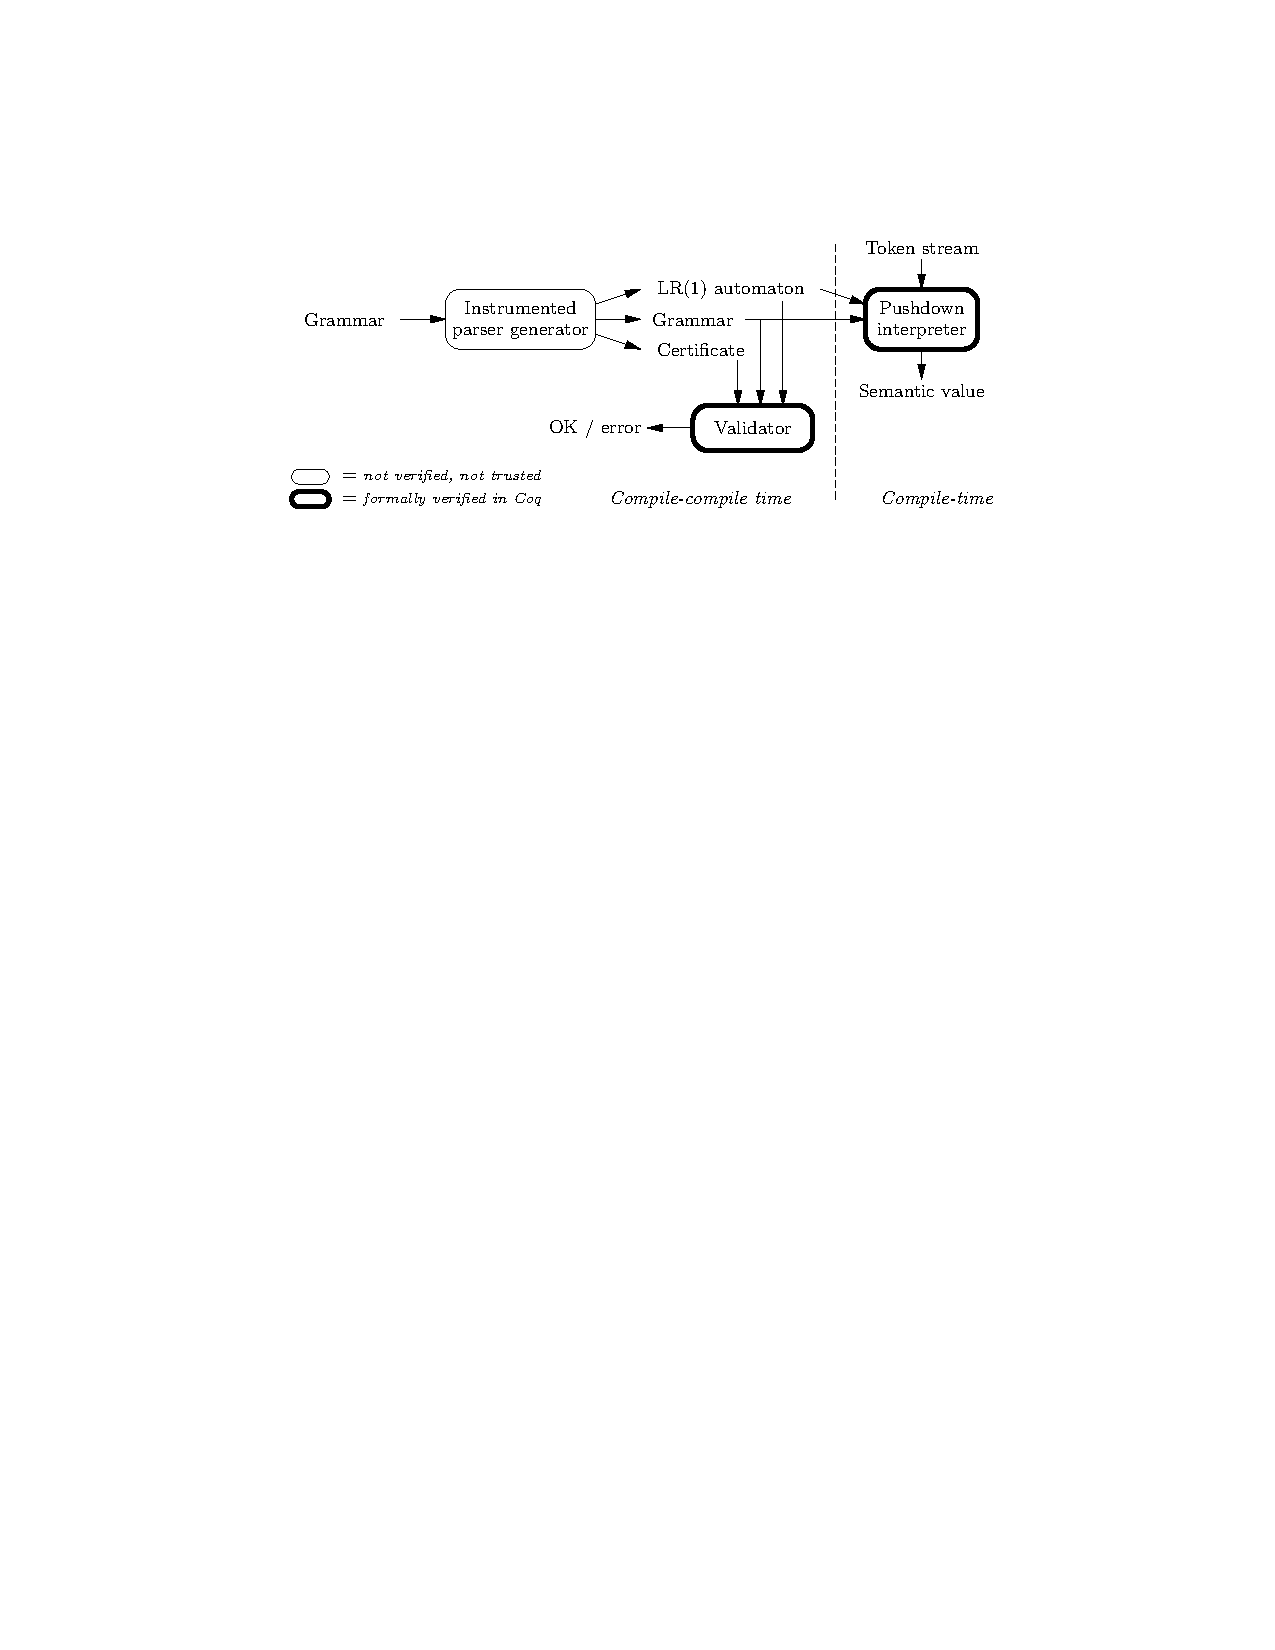
\includegraphics{figure}
\end{center}
\caption{General architecture.}
\label{fig-archi}
\end{figure}

There are many ways to build confidence in a parser.  Perhaps the
simplest way is to instrument an unverified parser so that it produces
full parse trees, and, at every run of the compiler, check that the
resulting parse tree conforms to the grammar.  This approach is easy
to implement but does not establish
completeness (all valid inputs are accepted)
or unambiguity (for each input, there is at most one parse tree).
Another approach is to apply program proof directly
to a hand-written or generated parser.  However, such a proof is
tedious, especially if the parser was automatically generated,
and must be re-done every time the the parser is
modified. Yet another approach, developed by Barthwal and
Norrish~\cite{barthwal-norrish-09,Barthwal-phd}, is to formally verify, once and
for all, a parser generator, guaranteeing that whenever the verified
generator succeeds, the parser that it produces is correct with respect to
the input grammar.  However, Barthwal and Norrish's proof is specific
to a particular parser generator that only accepts \slr grammars.  It
so happens that the ISO C99 grammar we are interested in is not \slr.
Before being applicable to CompCert, Barthwal and Norrish's work
would, therefore, have to be extended in nontrivial ways to a richer
class of grammars such as \lalr.

In this paper, we develop a fourth approach: {\em a posteriori}
verified validation of an \lrone automaton produced by an untrusted
parser generator, as depicted in Fig.~\ref{fig-archi}. After every run
of the parser generator (that is, at {\em compile-compile time\/}),
the source grammar $\grammar$, the generated automaton $\automaton$,
and auxiliary information acting as a certificate are fed in a {\em
validator}, which checks whether $\automaton$ recognizes the same
language as $\grammar$.  If so, the build of the compiler proceeds; if
not, it is aborted with an error.

The first contribution of this paper is the algorithm that performs
this validation. It is relatively simple, and, to the best of
our knowledge, original. It applies indifferently to many flavors of \lrone
automata, including \lrzero (a degenerate
case), \slr~\cite{deremer-slr-71}, \lalr~\cite{anderson-eve-horning-73},
Pager's method~\citeyear{pager-77}, and canonical \lrone~\cite{knuth-lr-65}.
The second contribution is a soundness proof for this algorithm,
mechanized using the Coq proof assistant, guaranteeing with the
highest confidence that if the validation of an automaton $\automaton$ against
a grammar~$\grammar$ succeeds, then the automaton~$\automaton$ and the interpreter
that executes it form a correct parser for $\grammar$. The last
contribution is an experimental assessment of our approach over the
ISO C99 grammar, demonstrating applicability to realistic parsers of
respectable size.

In summary, the approach to high-confidence parsing developed in this
paper is attractive for several reasons:
(1) it provides correctness guarantees about an \lrone parser as
strong as those obtained by verifying a \lrone parser generator;
(2) only the validator needs to be formally verified, but not the
parser generator itself, reducing the overall proof effort;
(3) the validator and its soundness proof are reusable with
different parser generators and different flavors of \lrone parsing;
(4) existing, mature parser generators such as Menhir~\cite{menhir} can be used
with minimal instrumentation, giving users the benefits of the
extensive diagnostics produced by these generators.

This paper is organized as follows. In \sref{sec:defs}, we review
context-free grammars, \lrone automata, and their meaning.
In \sref{sec:theorems}, we establish three properties of automata, namely
soundness (\sref{sec:soundness}), safety (\sref{sec:safety}) and completeness
(\sref{sec:completeness}). Safety and completeness are true only of some
automata: we present a set of conditions that are sufficient for these
properties to hold and that can be automatically checked by a validator.
After presenting some facts about our Coq implementation (\sref{sec:coq}), we
discuss its application to a C99 parser in the setting of CompCert
(\sref{sec:C}). We conclude with discussions of related work
(\sref{sec:related}) and directions for future work (\sref{sec:future}).

Our modifications to Menhir are available as part of the standard
release~\cite{menhir}.  Our Coq code is not yet part of the CompCert release,
but is available online~\cite{coq-code}.

\section{Grammars and Automata}
\label{sec:defs}

\subsection{Symbols}

We fix an alphabet of \emph{terminal symbols} $\term$ and an alphabet of
\emph{non-terminal symbols}~$\nonterm$, where
an \emph{alphabet} is a finite set. A \emph{symbol} $\sym$ is either a
terminal symbol or a non-terminal symbol.  We write~$\phrase$ for
a \emph{sentential form}, that is, a finite sequence of symbols.

\subsection{Grammars}

We fix a grammar $\grammar$, where a \emph{grammar} consists of:
\begin{enumerate}
\item a \emph{start symbol} $S$;
\item an alphabet of \emph{productions} $p$;
\item for every symbol $\sym$, a type $\sst\sym$.
\end{enumerate}
The first two components are standard. (The syntax of productions will be
presented shortly.)
The third component, which is not usually found in textbooks, arises because
we are interested not in recognition, but in parsing: that is, we would like
not only to decide whether the input is valid, but also to construct a
\emph{semantic value}. In other words, we would like to consider that a
grammar defines not just a \emph{language} (a set of words) but
a \emph{relation} between words and semantic values. However,
before we do so, we must answer the question:
%
what is the type of semantic values? It should be decided by the user, that
is, it should be part of the grammar. Furthermore, one should allow distinct
symbols to carry different types of semantic values. For instance, a terminal
symbol that stands for an identifier might carry a string, while a
non-terminal symbol that stands for an arithmetic expression might carry an
abstract syntax tree, that is, a value of a user-defined inductive type.  If
we were to force the user to adopt a single universal type of semantic values,
the user's code would become polluted with tags and dynamic tests, and it
would not be possible for the user to argue that these tests cannot fail. For
this reason, for every symbol~$\sym$, we allow the
user to choose the type $\sst\sym$ of the semantic values carried
by~$\sym$. (In Coq, $\sst\sym$ has type \verb+Type+.) By abuse of notation, if
$\phrase$ is a (possibly empty) sequence of symbols $\sym_1\ldots\sym_n$,
we write $\sst\phrase$ for the tuple type
$\sst{\sym_1}\times\ldots\times\sst{\sym_n}$.

How are semantic values constructed? The answer is two-fold. The semantic
values carried by terminal symbols are constructed by the lexer: in other
words, they are part of the input that is submitted to the parser. The
semantic values carried by non-terminal symbols are constructed by the parser:
when a production is reduced, a semantic action is executed. Let us now
examine each of these two aspects in greater detail.

The input of the parser is a stream of tokens, where a \emph{token} is a
dependent pair $(\term, \sv)$ of a terminal symbol $\term$ and a semantic
value $v$ of type~$\sst\term$. We assume that this stream is infinite. There
is no loss of generality in this assumption: if one wishes to work with a
finite input stream, one can complete it with an infinite number of copies of
a new ``end-of-stream'' token.
In the following, we write $\word$ for a finite sequence of tokens and
$\stream$ for an infinite stream of tokens.

A \emph{production} $p$ is a triple of the form
$\production\nonterm\phrase\sa$. (Above, we have written that productions form
an alphabet, that is, they are numbered. We abuse notation and elide the
details of the mapping from productions-as-numbers to productions-as-triples.)
The left-hand side of a production is a non-terminal symbol~$\nonterm$. The
right-hand side consists of a sentential form~$\phrase$ and a \emph{semantic
action}~$\sa$ of type $\sst\phrase\rightarrow\sst\nonterm$.
% In the Coq code, semantic actions are curried, but I don't think
% this matters.
The semantic action, which is provided by the user, indicates how a tuple of
semantic values for the right-hand side $\phrase$ can be transformed into a
semantic value for the left-hand side $\nonterm$. In our approach, the
semantic action plays a dual role: on the one hand, it is part of the grammar,
and plays a role in the definition of the semantics of the grammar; on the
other hand, it is used, at runtime, by the parser. The semantic action is a
Coq function and is supplied by the user as part of the grammar. (The parser
generator Menhir views semantic actions as pieces of text, so no modification
is needed for it to support Coq semantic actions instead of Objective Caml
semantic actions.)
% And Objective Caml and Coq have the same lexical conventions.

\subsection{Semantics of Grammars}

The semantics of grammars is usually defined in terms of a relation between
symbols $\sym$ and words $\word$, written $\hsv\sym\word{}$, pronounced:
``$\sym$~derives~$\word$''. As announced earlier, we extend this relation with
a third parameter, a semantic value~$\sv$ of type~$\sst\sym$. Thus, we
write $\hsv\sym\word\sv$, pronounced:
``$\sym$~derives~$\word$~producing~$\sv$''. The inductive definition of this
relation is as follows:
%
\begin{mathpar}
\inferrule{}
  {\hsv\term{(\term,\sv)}\sv}

\inferrule
  {
    \production\nonterm{\sym_1\ldots\sym_n}\sa \text{ is a production} \\\\
    \forall i \in\{1,\ldots,n\}
    \qquad
    \hsv{\sym_i}{\word_i}{\sv_i}
  }
  {\hsv\nonterm{\word_1\ldots\word_n}{\sa(\sv_1,\ldots,\sv_n)}}
\end{mathpar}
%

This semantics is used when we state that the parser is sound and complete
with respect to the grammar (Theorems~\ref{th:sound} and~\ref{th:complete}).

\subsection{Automata}
\label{sec:automata}

We fix an automaton~$\automaton$, where an \emph{automaton} consists of:
\begin{enumerate}
\item an alphabet of \emph{states} $\state$, with a distinguished
     \emph{initial state}, written $\Init$;
\item an action table;
\item a goto table;
\item for every non-initial state $\state$, an incoming symbol,
      written $\lss\state$.
\end{enumerate}

A \emph{non-initial state} is a state other than $\Init$.

An \emph{action table} is a total mapping of pairs $(\state,\term)$ to
actions. The idea is, if~$\state$ is the current state of the automaton and
$\term$ is the terminal symbol currently found at the head of the input
stream, then the corresponding action instructs the automaton what to do next.
%
An \emph{action} is one of
$\Ashift{\state'}$ (where $\state'$ is non-initial),
$\Areduce p$ (where $p$ is a production),
$\Aaccept$, and
$\Areject$.
%
In particular, the situation where the action table maps $(\state,\term)$ to
$\Ashift{\state'}$ can be thought of graphically as an edge, labeled $\term$,
from $\state$ to $\state'$.

% The definition of the automaton is relative to the (fixed) grammar:
% the symbols and productions are those of the grammar. Maybe we don't
% need to say this.

\begin{remark}
\label{remark:default}
  Our description of the action table as a mapping of pairs $(\state, \term)$
  to actions appears to imply that the parser \emph{must} peek at the next input
  token~$\term$ \emph{before} it can decide upon the next action. This might
  seem perfectly acceptable: because we have assumed that the input stream is
  infinite, there always is one more input token. In practice, however, more
  care is required. There are situations where the input stream is effectively
  infinite and nevertheless one must not allow the parser to systematically
  peek at the next token. For instance, the input stream might be connected to
  a keyboard, where a user is entering commands. If the parser has been asked
  to recognize one command, then, upon finding the end of a command, it should
  terminate and report success \emph{without} attempting to read one more
  token: otherwise, it runs the risk of blocking until further keyboard input
  is available!

  In order to address this problem, we allow our automata to sometimes
  take a \emph{default action} without peeking at the next input
  token. We adopt the following convention: if, for a certain state $\state$
  and for all terminal symbols $\term$, the entries found at $(\state,\term)$
  in the action table are identical, then the automaton, when in
  state~$\state$, determines which action should be taken \emph{without}
  consulting the input stream\footnote{Of course, it would be inefficient to
  naïvely test whether one entire column of the action table contains
  identical entries. In reality, Menhir produces (and our Coq code
  uses) a two-level action table, where the first level is indexed only by a
  state~$\state$ and indicates whether there exists a default action, and the
  second level (which is consulted only if there is no default action) is
  indexed by a state~$\state$ and a terminal symbol~$\term$.}.
  % (A default action is always a \emph{reduce} or \emph{accept} action.)
\end{remark}

A \emph{goto table} is a partial mapping of pairs $(\state,\nonterm)$ to
non-initial states. If the goto table maps $(\state,\nonterm)$ to $\state'$,
then the automaton can take a transition from~$\state$ to $\state'$ after
recognizing a word that derives from $\nonterm$. This can be thought of
graphically as an edge, labeled $\nonterm$, from $\state$ to $\state'$. This
table is a partial mapping: a state $\state$ may have no outgoing edge labeled
$\nonterm$.

A well-formed \lr automaton has the property that, for every non-initial state
$\state$, all of the edges that enter $\state$ carry a common label. (The
initial state $\Init$ has no incoming edges.) We refer to this label as
the \emph{incoming symbol} of~$\state$. Although we could have our validator
reconstruct this information, we ask the user to supply it as part of the
description of the automaton. We require that this information be consistent
with the action and goto tables, as follows.
%
If the action table maps $(\state,\term)$ to $\Ashift{\state'}$, then we
require $\lss{\state'}=\term$. Similarly, if the goto table maps
$(\state,\nonterm)$ to $\state'$, then we require $\lss{\state'}=\nonterm$.
We encode these requirements directly in the types of the action and goto
tables, using dependent types, so we do not need to write validation code
for them.
% These properties allow us to suppress some dynamic checks in the interpreter.

\subsection{Semantics of Automata}
\label{sec:interpreter}

We give semantics to automata by defining an interpreter for automata. The
interpreter is a function named $\parse\cdot\cdot$. Its first (and main)
argument is a token stream $\stream$. We need an auxiliary argument, the
``fuel'', which is discussed further on.

The interpreter maintains a \emph{stack} $\stack$, which is a list of dependent pairs
of a non-initial state~$\state$ and a semantic value $\sv$ of type
$\sst{\lss\state}$. Indeed, $\lss\state$ is the (terminal or non-terminal)
symbol that was recognized prior to entering state $\state$, and $\sv$ is a
semantic value associated with this symbol.
%
% Notation utilisée une fois un peu plus loin.
We write $\Cons{\stack}{\state}{\sv}$ for a stack whose top cell is the pair
$(\state,\sv)$ and whose tail is the stack $\stack$.
%
At the beginning of a run, the
stack is empty. At every moment, the \emph{current state} of the automaton
is the state found in the top stack cell if the stack is non-empty; it is
the initial state $\Init$ if the stack is empty%
\footnote{In many textbooks, one does not consider semantic
values, so the stack is a list of states; at the beginning of a run,
the stack is a singleton list of the state $\Init$; the stack is never
empty, so the current state is always the one found on top of the stack.}.

In several places, the interpreter can generate an internal error, revealing a
flaw in the automaton. Indeed, it is sometimes much easier to write an
interpreter that can encounter an internal error, and prove \emph{a
posteriori} that this situation never arises if the automaton satisfies
certain properties, than to define \emph{a priori} an interpreter than never
encounters an internal error. In other words, instead of
hardwiring \emph{safety} (that is, the absence of internal errors) into the
definition of the interpreter, we make it a separate theorem
(Theorem~\ref{th:safety}).

We use an error monad to deal with internal errors. In this paper, we use
$\Err$ to denote an internal error. By abuse of notation, we elide the
``return'' operation of the error monad. Thus, the interpreter produces either
$\Err$ or a parse result (defined below).

We also need a way of dealing with the possibility of non-termination. Again,
it is not possible to prove \emph{a priori} that the interpreter terminates.
When an \lr automaton reduces a unit production (of the form
$\produ\nonterm{\nonterm'}$) or an epsilon production (of the form
$\produ\nonterm\epsilon$), the size of the stack does not decrease.
There do exist automata, as per the definition of \S\ref{sec:automata}, whose
interpretation does not terminate. It is not clear, at present, what property
one could or should require of the automaton in order to ensure
termination. (We discuss this issue in \S\ref{sec:future}.)

We adopt a simple and pragmatic approach to this problem: in addition to the
token stream, the interpreter requires an integer argument $n$, which we
refer to as the \emph{fuel}.  In the main loop of the interpreter,
each iteration consumes one unit of fuel.  If the interpreter runs out of
fuel, it stops and reports that it was not able to terminate normally.
We write $\Rtimeout$ for this outcome.

Thus, a \emph{parse result} is one of: $\Rtimeout$, which was explained above;
$\Rreject$, which means that the input is invalid; and $\Rparsed\sv\stream$,
which means that the input is valid, that the semantic value associated with
the prefix of the input that was recognized is $\sv$, and that the remainder
of the input is $\stream$. (The value~$\sv$ has type $\sst{S}$, where $S$ is
the start symbol of the grammar. The value $\stream$ is a token stream.)

In summary, the interpreter accepts a token stream and a certain amount of
fuel and produces either $\Err$ or a parse result, as defined above.

The interpreter works in a standard manner. At each step, it looks up the
action table at $(\state,\term)$, where $\state$ is the current state of the
automaton and $(\term,\sv)$ is the next input token.
% (see Remark~\ref{remark:default} for details).
Then,
\begin{enumerate}
\item if the action is $\Ashift{\state'}$,
      the input token $(\term,\sv)$ is consumed, and
      the new cell $(\state',\sv)$ is pushed onto the stack.
      Because $\lss{\state'}=\term$ holds, it is possible to
      \emph{cast} the value $\sv$ from the
      type $\sst\term$ to the type $\sst{\lss{\state'}}$: this is required
      for this new stack cell to be well-typed.
      % When the interpreter is extracted to OCaml code, the cast is erased.
\item if the action is $\Areduce
      {\production\nonterm{\sym_1\ldots\sym_n}\sa}$, the interpreter
      \emph{attempts} to pop~$n$ cells off the stack, say $(\state_1,\sv_1)\ldots(\state_n,\sv_n)$, and
      \emph{dynamically checks} that $\lss{\state_i}=\sym_i$ holds for every $i\in\{1,\ldots,n\}$. If
      the stack does not have at least $n$ cells, or if this check fails,
      then an internal error occurs. Otherwise, thanks to the
      success of these dynamic checks, each of the semantic values $\sv_i$
      can be cast from the type $\sst{\lss{\state_i}}$ to the
      type $\sst{\sym_i}$. Thus, the tuple $(\sv_1,\ldots,\sv_n)$ admits
      the type $\sst{\sym_1\ldots\sym_n}$, and is a suitable argument for
      the semantic action~$\sa$. The application of $\sa$ to this tuple
      yields a new semantic value $\sv$ of type~$\sst\nonterm$. There
      remains for the interpreter to consult the goto table at the current state and at
      the non-terminal symbol $\nonterm$. If this entry in the goto
      table is undefined, an internal error occurs. Otherwise, this entry
      contains a state $\state'$, and (after another cast) the new cell
      $(\state',\sv)$ is pushed onto the stack.
\item if the action is $\Aaccept$, the interpreter attempts to pop one cell off
      the stack, say $(\state,\sv)$, and checks that $\lss\state=S$ holds,
      where $S$ is the start symbol of the grammar. Thus, the value $\sv$
      can be cast to the type $\sst{S}$. (This can be thought of as
      reducing a special production $\produ{S'}{S}$.) The
      interpreter then checks that the stack is now empty
      % (again causing an internal error if this is not the case)
      and terminates with the parse result $\Rparsed\sv\stream$,
      where $\stream$ is what remains of the input stream.
      % @JH: le test $\lss\state=S$ pourrait aussi être codé en dur dans le type
      % de la table des actions. (On n'y gagnerait certes pas grand-chose.)
\item if the action is $\Areject$, the interpreter stops
      with the parse result $\Rreject$.
\end{enumerate}

In summary, there are four possible causes for an internal error: a dynamic
check of the form $\lss\state=\sym$ may fail; an attempt to pop a cell off
the stack fails if the stack is empty; an attempt to consult the goto table
fails if the desired entry is undefined; an attempt to accept fails if the
stack is nonempty.
% about 200 loc

\section{Correctness Properties and Validation}
\label{sec:theorems}

We now show how to establish three properties of the automaton $\automaton$
with respect to the grammar $\grammar$. These properties are \emph{soundness}
(the parser accepts only valid inputs), \emph{safety} (no internal error
occurs), and \emph{completeness} (the parser accepts all valid inputs). By
design of our interpreter, the first property is true of all automata, whereas
the latter two are true only of some automata. For safety and for
completeness, we present a set of conditions that are sufficient for the
desired property to hold and that can be automatically checked by a validator.

\subsection{Soundness} 
\label{sec:soundness}

The soundness theorem states that if the parser accepts a finite prefix
$\word$ of the input stream $\stream$, then (according to the grammar) the
start symbol $S$ derives $\word$. More precisely, if the parser accepts
$\word$ and produces a semantic value $\sv$, then $\sv$ is the value
associated with this particular derivation of $\word$ from $S$, that is, the
relation $\hsv{S}\word\sv$ holds.
%
\begin{theorem}[Soundness]
\label{th:sound}
If $\parse{\stream}{n} = \Rparsed\sv{\stream'}$ holds, then there exists a
word $\word$ such that $\stream = \word \stream'$ and $\hsv{S}{\word}{\sv}$.
\end{theorem}

No hypotheses about the automaton are required, because the situations where
``something is wrong'' and soundness might be endangered are detected at
runtime by the interpreter and lead to internal errors. In other words, we
have shifted most of the burden of the proof from the soundness theorem to the
safety theorem.

In order to prove this theorem, it is necessary to establish an invariant
stating that the symbols associated with the states found in the stack derive
the input word that has been consumed. For this purpose, we introduce a new
predicate, written $\stack\Longrightarrow\word$, which relates a stack
$\stack$ with a token word $\word$. It is inductively defined as follows:
%
\begin{mathpar}
\inferrule{}
  {\Nil \Longrightarrow \epsilon}

\inferrule{
  \stack \Longrightarrow \word_1 \\
  \hsv{\lss{\state}}{\word_2}{\sv}
}{
  \Cons{\stack}{\state}{\sv} \Longrightarrow \word_1\word_2
}
\end{mathpar}
%
Then, the main soundness invariant can be stated as follows: if the parser has
consumed the input word $\word$ and if the current stack is $\stack$, then
$\stack \Longrightarrow \word$ holds.

\subsection{Safety}
\label{sec:safety}

The safety theorem states that if the automaton passes the \emph{safety
  validator} (which we describe further on) then the interpreter never
encounters an internal error. A \emph{validator} is a Coq term of type
\verb+bool+, which has access to the grammar, to the automaton, and to certain
additional annotations that serve as hints (and which we describe below as
well). Thus, the safety theorem takes the following form:
%
\begin{theorem}[Safety]
\label{th:safety}
If the criteria enforced by the safety validator are satisfied, then
$\parse{\stream}{n} \neq \Err$ for every
input stream $\stream$ and for every integer ``fuel''~$n$.
\end{theorem}

All of the causes of internal errors that were previously listed
(\sref{sec:interpreter}) have to do with a stack that does not
have the expected shape (e.g., it has too few cells) or contents
(e.g. some cell contains a semantic value of inappropriate type,
or contains a state for which no entry exists in the goto table).
% Le cas de l'action accept est particulier, je crois: on y exige
% que la pile soit vide; or cela ne découle pas de l'invariant sur
% la pile, dont nous allons parler maintenant, mais du fait que
% accept n'est permis que dans l'état init, et du fait que l'état
% init n'a aucun prédécesseur, donc la pile y est forcément vide.
Thus, in order to ensure safety, we must have precise control
of the shape and contents of the stack.

Recall that a stack~$\stack$ is a sequence of pairs
$(\state_1,\sv_1)\ldots(\state_n,\sv_n)$. In what follows, it is convenient to
abstractly describe the structure of such a stack in two ways. First, we are
interested in the underlying sequence of symbols: we write
$\symsOfStack\stack$ for the sequence of symbols
$\lss{\state_1}\ldots\lss{\state_n}$. Second, we are interested in the
underlying sequence of states: we write $\statesOfStack\stack$ for the
sequence of singleton sets $\{\Init\}\{\state_1\}\ldots\{\state_n\}$. (We use
singleton sets here because we will shortly be interested in approximating
these singleton sets with larger sets of states~$\State$.)
% A set of states $\State$ will be interpreted as a disjunction... (Obvious?)

A key remark is the following: the sequences $\symsOfStack\stack$ and
$\statesOfStack\stack$ are not arbitrary. They follow certain patterns, or, in
other words, they respect a certain invariant. This invariant will be
sufficient to guarantee safety.

How do we find out what this invariant is? Two approaches come to mind: either
the safety validator could reconstruct this invariant by performing a static
analysis of the automaton (this would require a least fixed point
computation), or the parser generator could produce a description of this
invariant, which the safety validator would verify (this would require
checking that a candidate fixed point is indeed a fixed point). We somewhat
arbitrarily adopt the latter approach. The former approach appears viable as
well, especially if one exploits a pre-existing verified library for computing
least fixed points.

Thus, the annotations that the safety validator requires (and that the parser
generator must produce) form a description of the safety invariant.  For each
non-initial state~$\state$, these annotations are:
\begin{enumerate}
\item a sequence of symbols, written $\pss\state$;
\item a sequence of sets of states, written $\psts\state$.
\end{enumerate}
(There is a redundancy, which we discuss in \sref{sec:future}.)
% francois: c'est redondant, car un "incoming symbol" est équivalent à un
% ensemble d'états.
% Jh : oui, effectivement. C'est clairement un point où les annotations
% pourraient être plus petites. En plus, ça pourrait simplifier le
% validateur. Pour la version finale, peut-être.
These annotations are meant to represent approximate (conservative)
information about the shape and contents of the stack. In order to explain
their meaning, let us now define the safety invariant in terms of these
annotations.

We begin by defining the relations that exist between abstract descriptions of
the stack and concrete stacks. We need two such relations. The \emph{suffix
  ordering} between two \emph{sequences of symbols} is defined in the usual
way: that is, $\sym_m\ldots\sym_1$ is a suffix of $\sym'_n\ldots\sym'_1$ if
and only if $m\leq n$ holds and $\sym_i=\sym'_i$ holds for every
$i\in\{1,\ldots,m\}$. The \emph{suffix ordering} between two \emph{sequences
  of sets of states} is defined in the same manner, up to pointwise superset
ordering: that is, $\State_m\ldots\State_1$ is a suffix of
$\State'_n\ldots\State'_1$ if and only if $m\leq n$ and
$\State_i\supseteq\State'_i$ holds for every $i\in\{1,\ldots,m\}$.

Equipped with these suffix orderings, which serve as abstraction
relations, we can define the safety invariant. This is a predicate
over a stack, written $\stackinv\stack$. It is inductively defined
as follows:
%
\begin{mathpar}
\inferrule{}{\stackinv\Nil}
  
\inferrule{
  \pss\state \text{ is a suffix of } \symsOfStack\stack \\\\
  \psts\state \text{ is a suffix of } \statesOfStack\stack \\\\
  \stackinv\stack
}{
  \stackinv{\stack(\state,\sv)}
}
\end{mathpar}

A stack $\stack(\state,\sv)$ is safe if (a) the annotations $\pss\state$ and
$\psts\state$ associated with the current state~$\state$ are correct
approximate descriptions of the tail~$\stack$ of the stack and (b) the tail
$\stack$ is itself safe.
%
Less formally, $\pss\state$ and $\psts\state$ are static descriptions of a
suffix of the stack (i.e., the part of the stack that is closest to the top).
The rest of the stack, beyond this statically known suffix, is unknown.
Nevertheless, this information is sufficient (if validation succeeds) to show
that internal errors cannot occur: for instance, it guarantees that, whenever
we attempt to pop $k$ cells off the stack, at least $k$ cells are present.

Now, in order to ensure that $\stackinv\stack$ is indeed an invariant of the
interpreter, the validator must check that the annotations $\pss\state$ and
$\psts\state$ are consistent. Furthermore, the validator must verify a few
extra conditions which, together with the invariant, ensure safety. The
safety validator checks that the following properties are satisfied:
%
\begin{enumerate}
\item For every transition, labeled $\sym$, of a state $\state$ to a new state $\state'$,
      % that is, either $\sym$ is a terminal and the action table maps
      % $(\state, \sym)$ to $\Ashift{\state'}$, or $\sym$ is a non-terminal and
      % the goto table maps $(\state, \sym)$ to $\state'$)
      % -- déjà dit plus haut
     \begin{itemize}
     \item $\pss{\state'}$ is a suffix of $\pss\state\lss{\state}$,
     \item $\psts{\state'}$ is a suffix of $\psts\state\{\state\}$.
     \end{itemize}
\item For every state $\state$ that has an action of the form
      $\Areduce{\production\nonterm\phrase\sa}$,
     \begin{itemize}
     \item $\phrase$ is a suffix of $\pss\state\lss{\state}$,
     \item If $\psts\state\{\state\}$ is $\State_n\ldots\State_0$
           and if the length of $\phrase$ is $k$, then
           for every state $\state' \in \State_k$, the
           goto table is defined at $(\state', \nonterm)$.
           (If $k$ is greater than~$n$, take $\State_k$ to
           be the set of all states.)
           % fpottier: on pourrait supprimer cette parenthèse en imposant
           % (i.e. en validant que) $k\leq n$?
           % Je serais surpris que l'automate tente de réduire au-delà du
           % segment de pile connu.
           % Ou bien, comme le reviewer 1 l'a noté, il suffirait de valider
           % que pastStates et pastSymbols ont la même longueur pour avoir
           % $k \leq n$. A fortiori, le problème disparaîtrait si on
           % supprimait la redondance entre pastStates et pastSymbols.
     \end{itemize}
\item For every state $\state$ that has an $\Aaccept$ action,
      % Accept is always a default action.
     \begin{itemize}
       \item $\state \neq \Init$,
       \item $\lss\state = S$,
       \item $\psts\state = \{\Init\}$.
     \end{itemize}
\end{enumerate}

Thanks to the finiteness of the alphabets, these conditions are clearly and
efficiently decidable.

These conditions do not depend in any way on the manner in which lookahead is
exploited to determine the next action. In other words, an \lrone automaton is
safe if and only if the underlying non-deterministic \lrzero automaton is
safe. Thus, the safety validator is insensitive to which method was used to
construct the \lrone automaton.

% ----------------------------------------------------------------------------

\subsection{Completeness}
\label{sec:completeness}

The completeness theorem states that if the automaton passes
the \emph{completeness validator} (which we describe further on), if a prefix
$\word$ of the input is valid, and if enough fuel is supplied, then the
parser accepts $\word$ and constructs a correct semantic value. (The theorem
also allows for the possibility that the parser might encounter an internal
error. This concern was dealt with in \S\ref{sec:safety}, so we need not worry
about it here.)

% \begin{theorem}[Weak completeness]
% If the criteria enforced by the completeness validator are satisfied and
% if $\hsv{S}\word\sv$ holds, then
% for every $\stream$ and $n$, either
% $\parse{\word\stream}{n} \in \{\Err, \Rtimeout\}$ or
% $\parse{\word\stream}{n} = \Rparsed\sv\stream$.
% \end{theorem}

\begin{theorem}[Completeness]
\label{th:complete}
If the criteria enforced by the completeness validator are satisfied and
if $\hsv{S}\word\sv$ holds, then
there exists $n_0$ such that
for all~$\stream$ and for all $n\geq n_0$, either
$\parse{\word\stream}{n} = \Err$ or
$\parse{\word\stream}{n} = \Rparsed\sv\stream$.
\end{theorem}
% J'ai affaibli l'énoncé de JH, qui disait que si on appelle le parser avec
% $n < n_0$, alors on peut en plus avoir $\Rtimeout$. C'est une conséquence
% de l'énoncé ci-dessus et d'un lemme de monotonie (qui affirme que si on
% donne moins de fuel, on aura soit le même résultat, soit $\Rtimeout$).

The Coq version of this result is in fact more precise. We prove that a
suitable value of~$n_0$ is the size of the derivation tree for the hypothesis
$\hsv{S}\word\sv$, and we prove that this is the least suitable value, that
is, $n<n_0$ implies $\parse{\word\stream}{n} = \Rtimeout\,$.

% ----------------------------------------------------------------------------

% What information does the completeness validator require?
In order to guarantee that the automaton is complete, the validator must check
that each state has ``enough'' permitted actions for every valid input to be
eventually accepted. But how do we know, in a state $\state$, which actions
should be permitted? We can answer this question if we know which set
of \lrone items is associated with $\state$.
%
Recall that an \emph{item} is a quadruple
$\lritem\nonterm{\phrase_1}{\phrase_2}\term$, where
$\production\nonterm{\phrase_1\phrase_2}\sa$ is a production and $\term$ is a
terminal symbol.
%
% which we refer to as the \emph{lookahead symbol} of this item.
%
The intuitive meaning of an item is: ``we have recognized $\phrase_1$; we now
hope to recognize $\phrase_2$ and find that it is followed with $\term$; if
this happens, then we will be able to reduce the production
$\production\nonterm{\phrase_1\phrase_2}\sa$''.

Our items are relative to an \emph{augmented} grammar, where a virtual
production $\produ{S'}{S}$ has been added. This means that we can have items
of the form $\lritem{S'}{}{S}\term$ (these appear in the initial
state of the automaton) and items of the form $\lritem{S'}{S}{}\term$ (these
appear in the final, accepting state).

The parser generator knows which set of items is associated with each state of
the automaton. We require that this information be transmitted to the
completeness validator. (One could instead reconstruct this information, and
one would not even need to prove the correctness of the algorithm that
reconstructs it;
% but one would need to prove its termination!
but it is not clear what one would gain by doing so.)

With this information, the validator carries out two kinds of checks. First,
it checks that each state $\state$ has ``enough'' actions: that is, the
presence of certain items in $\items\state$ implies that certain actions must
be permitted. Second, it checks that the sets $\items\state$ are \emph{closed}
and \emph{consistent}: that is, the presence of certain items in
$\items\state$ implies that certain items must be present in $\items\state$
(this is \emph{closure}) and in $\items{\state'}$, where $\state'$ ranges over
the successor states of~$\state$ (this is \emph{consistency}).

The definition of the closure property, which appears below, relies on
the knowledge of the ``\textit{first}'' sets, which in turn requires the
knowledge of which non-terminal symbols are ``\textit{nullable}''. It is
well-known that ``\textit{first}'' and ``\textit{nullable}'' form the least
fixed point of a certain system of positive equations. Again, we could have
the validator compute this least fixed point; instead, we require that it be
transmitted from the parser generator to the validator, and the validator just
checks that it is a fixed point.

% By definition, $\nullable\phrase$ is true if and only if $\phrase$ derives
% the empty word.

% By definition, $\term\in\first\phrase$ is true if and only if $\phrase$
% derives a word of the form $\term\word$.

In summary, the annotations that the completeness validator requires (and that
the parser generator must produce) are:
\begin{enumerate}
\item for each state $\state$, a set of items, written $\items\state$.
\item for each non-terminal symbol $\nonterm$, a set of terminal symbols $\first\nonterm$;
\item for each non-terminal symbol $\nonterm$, a Boolean value $\nullable\nonterm$.
\end{enumerate}

% ----------------------------------------------------------------------------

% What properties does the completeness validator check?

The properties that the completeness validator enforces are:
%
\begin{enumerate}
\item ``\textit{first}'' and ``\textit{nullable}'' are fixed points of the standard
      defining equations.
\item For every state $\state$, the set $\items\state$ is closed, that is, the
      following implication holds:
      \begin{mathpar}
      \inferrule{
        \lritem\nonterm{\phrase_1}{\nonterm'\phrase_2}\term \in \items\state \\\\
        \production{\nonterm'}{\phrase'}{\sa'} \text{ is a production} \\\\
        \term' \in \first{\phrase_2\term}
      }{
        \lritem{\nonterm'}{}{\phrase'}{\term'} \in \items\state
      }
      \end{mathpar}
\item For every state $\state$, if $\lritem\nonterm\phrase{}\term \in
      \items\state$, where $\nonterm \neq S'$, then
      the action table maps $(\state, \term)$ to
      $\Areduce{\production\nonterm\phrase\sa}$.
      % L'action sémantique $\sa$ semble parachutée, c'est flou, mais
      % on comprend (j'espère) qu'en réalité les productions sont
      % numérotées et il n'y a aucun problème.
\item For every state $\state$, if
      $\lritem\nonterm{\phrase_1}{\term\phrase_2}{\term'} \in \items\state$, then
      the action table maps $(\state, \term)$ to $\Ashift{\state'}$, for some
      state $\state'$ such that:
      \[\lritem\nonterm{\phrase_1\term}{\phrase_2}{\term'}\in \items{\state'}\]
\item For every state $\state$, if
      $\lritem\nonterm{\phrase_1}{\nonterm'\phrase_2}{\term'} \in \items\state$,
      then the goto table
      either is undefined at $(\state, \nonterm')$
      or maps $(\state, \nonterm')$ to some state $\state'$ such that:
      \[\lritem\nonterm{\phrase_1\nonterm'}{\phrase_2}{\term'}\in \items{\state'}\]
      % On pourrait noter qu'exiger que la table goto soit définie est une
      % condition nécessaire pour la sûreté, pas pour la complétude.
\item For every terminal symbol $\term$, we have $\lritem{S'}{}S\term \in \items\Init$.
\item For every state $\state$, if $\lritem{S'}S{}\term \in \items\state$, then
      $\state$ has a default $\Aaccept$ action.
\end{enumerate}

These conditions are clearly decidable. In order to achieve reasonable
efficiency, we represent items in a compact way: first, we group items that
have a common \lrzero core; second, we use a natural number to indicate the
position of the ``bullet''. Thus, in the end, we manipulate triples of a
production identifier~$p$, an integer index into the right-hand side of $p$,
and a set of terminal symbols. Furthermore, we use the standard
library \texttt{FSets}~\cite{Filliatre-Letouzey-04}, which implements finite
sets in terms of balanced binary search trees, in order to represent sets of
items.

The various known methods for constructing \lrone automata differ only in how
they decide to merge, or not to merge, certain states that have a
common \lrzero core. The completeness validator is insensitive to this aspect:
as long as no conflict arises due to excessive merging, an arbitrary merging
strategy can be employed.
% Je crois que je veux dire quelque chose comme: si on a un automate qui passe
% le validateur et si on merge des états (sans faire apparaître de conflits)
% pour obtenir un nouvel automate, alors celui-ci passera aussi le validateur.
% En particulier, l'automate LR(1) canonique passe le validateur (on en est
% convaincus...) donc n'importe quel autre aussi.

% ----------------------------------------------------------------------------

% Idée de la preuve.

There is a relatively simple intuition behind the proof of
Theorem~\ref{th:complete}. Suppose an oracle gives us a proof of
$\hsv{S}\word\sv$, that is, a parse tree. Then, the parser, confronted with
the input $\word$, behaves in a very predictable way: it effectively performs
a depth-first traversal of this parse tree. When the parser performs
a \textit{shift} action, it visits a (terminal) leaf of the parse tree; when
it performs a \text{reduce} action, it visits a (non-terminal) node
of the parse tree. At any time, the parser's stack encodes the path that leads
from the root of the tree down
to the current node of the traversal, and holds the semantic values associated
with parse tree nodes that have been fully processed, but whose parent has not
been fully processed yet. At any time, the unconsumed input corresponds to the
fringe of the part of the parse tree that has not been traversed yet.

% Nouveau paragraphe en version finale.
This invariant allows us to prove that the parser cannot reject the input
$\word\stream$. Instead, it keeps shifting and reducing until it has traversed
the entire parse tree. At this point, it has consumed exactly $\word$, and it
must accept and produce exactly $\sv$. Note that there is no need to implement
an ``oracle''. We simply prove that if \emph{there exists} a parse tree, then
the parser behaves \emph{as if} it were traversing this parse tree, and
accepts at the end.

In order to make this intuition precise, we define an invariant that relates
the stack, the unconsumed input, and a path in the parse tree provided by the
``oracle''. The definition of this invariant is quite technical, but can be
summed up as follows. There exists a path in the ``oracle'' parse tree such
that:
% In fact, defining this invariant was the main difficulty.
%
\begin{enumerate}
\item The path begins at the root of the parse tree.
\item For each node in this path, the children of this node can be divided
      in three consecutive segments (or, at the last node in the path, in two segments):
      \begin{itemize}
      \item children that have already been visited: the semantic value associated with
            each of these children is stored in a stack cell;
      \item the child that is being visited (absent if we are at the
            bottom of the path): this child is the next node in the path;
      \item children that will be visited in the future: their fringes correspond
            to segments of the unconsumed input stream.
      \end{itemize}
\item The unconsumed input begins with the concatenation of the fringes of
      the ``unvisited children'' of all nodes in the path.
      % The unconsumed input is infinite, so it does not ``coincide'' with
      % the fringe, it only ``begins'' with the fringe.
      % concatenation de gauche à droite et de bas en haut.
\item The sequence of all stack cells is in one-to-one correspondence with
      the concatenation of the sequences of ``visited children'' of all nodes
      in the path.
      % concatenation de droite à gauche et de bas en haut.
\item As per the previous item, each
      stack cell $(\state, \sv)$ is associated with a certain child~$y$ of a
      certain node~$x$ in the path.
      Then, the semantic value carried by the node~$y$ must be precisely~$v$.
      Furthermore, if the node~$x$ is labeled with the production
      $\produ\nonterm{\phrase_1\sym\phrase_2}$ and if the child~$y$
      corresponds to the symbol~$\sym$,
      then the item $\lritem\nonterm{\phrase_1\sym}{\phrase_2}\term$
      appears in $\items\state$,
      where~$\term$ is the first symbol in the partial fringe
      that begins ``after'' the node $x$.
\end{enumerate}
During parsing, this path evolves in the following ways:
\begin{enumerate}
\item Between two actions: if the first unvisited child
  of the last node of the path exists and is not a terminal leaf, then the
  next action of the automaton will take place under this child. It is then
  necessary to extend the path: this child becomes the last node of the
  path. This extension process is repeated as many times as possible.
\item When shifting: if the first unvisited child of the last node exists and is a terminal leaf, then
  the next action must be a \textit{shift} action. This child is considered
  visited and transferred to the first segment of children of the last node.
  The path itself is unchanged. % au sens où la liste des noeuds qui constituent le chemin ne change pas.
\item When reducing: if the last node of the path has no unvisited child,
  then the next action must be a \textit{reduce} action for the production
  that corresponds to this node. Then, the path is shortened by one node:
  that is, if $x$ and $y$ are the last two nodes in the path, then $x$
  becomes the last node in the path, and $y$ becomes the last visited child of $x$.
\end{enumerate}

% These considerations us enable to prove that this invariant is preserved, and
% make the proof go through.

\subsection{Unambiguity}

It is easy to prove the following result.

\begin{theorem}
  Suppose there exists a token.
  % Il faut qu'il existe au moins un symbole terminal (c'est vraiment important)
  % et au moins une valeur sémantique pour ce symbole (c'est plus technique que réellement nécessaire).
  % Le token en question sert à construire le stream $\stream$ arbitraire ci-dessous.
  If the criteria enforced by the safety and completeness validators are
  satisfied, then the grammar is unambiguous.
\end{theorem}

The proof goes as follows.
%
Suppose that the automaton is safe and complete. Suppose further that, for
some word $\word$, both $\hsv{S}\word{\sv_1}$ and $\hsv{S}\word{\sv_2}$
hold. By the safety hypothesis, the parser never encounters an internal error
$\Err$. Thus, by the completeness hypothesis, given a sufficiently large
amount of fuel, the parser, applied to $\word\stream$ (where $\stream$ is
arbitrary), must produce $\sv_1$, and by a similar argument, must produce
$\sv_2$. However, our automata are deterministic by definition: \textit{parse}
is a function. Thus, $\sv_1$ and $\sv_2$ must coincide.

% Furthermore, parse is a monotonic function, in the sense that providing more
% fuel leads to a better-defined result (with respect to the flat ordering
% whose least element is $\Rtimeout$).

\section{Coq Formalization}
\label{sec:coq}

All of the results presented in this paper were mechanized using the
Coq~8.3pl1 proof assistant. The Coq formalization is fairly close to the
definitions, theorems and proofs outlined in this paper.

% It makes heavy use of the theory \verb|FSets| (part of Coq's standard
% library) to represent finite sets and finite maps in an efficient manner, to
% wit, as AVL trees~\cite{Filliatre-Letouzey-04}.

We use of dependent types to support semantic values and semantic actions
whose types are functions of the corresponding symbols and productions.  This
enables us to support user-supplied semantic actions with essentially no proof
overhead compared with a ``pure'' parser that only produces a parse tree.

We make good use of Coq's module system: the validator and
the interpreter are functors parameterized over abstract types for terminal
and non-terminal symbols. The only constraints over these two types of symbols
are that they must be finite (so that it is possible to decide universal
quantifications over symbols) and they must come with a decidable total order
(so that they can be used in conjunction with the \verb|FSets| library).

The Coq formalization is pleasantly small: about 2500 lines, excluding
comments.  The executable specifications of the safety validator and
the completeness validator are about 200 lines each.  The proofs of
soundness, safety, and completeness account for 200, 500, and 700
lines, respectively.

\section{Experimentation on a C99 Parser}
\label{sec:C}

% We evaluate the effectiveness of our validator on a parser for the
% latest version (ISO C99) of the C~programming language.

\paragraph{The grammar.} Our starting point is the context-free
grammar given in Annex~A of the ISO C99 standard \cite{ISO-C99}.  We
omit the productions that support unprototyped ``K\&R-style''
function definitions, since such old-style definitions are considered
``an obsolescent feature'' \cite[section 6.11.7]{ISO-C99} and are not
supported by subsequent passes of the CompCert compiler.  

Both this slightly simplified C grammar and the original ISO C99
grammar are ambiguous. There are three distinct sources of ambiguity.

The first source of ambiguity is the classic ``dangling-else'' problem, which
introduces a shift-reduce conflict in the \lrone automaton.  We eliminated
this conflict by a slight modification to the grammar, distinguishing two
non-terminal symbols for statements: one that prohibits \texttt{if} statements
without an \texttt{else} part, and the other that permits them.

The second source of ambiguity is the well-known problem with typedef
names (identifiers bound to a type by a \texttt{typedef}
declaration), which must be distinguished from other identifiers.
For example, ``\verb|a * b;|'' is to be parsed as a declaration of a
variable \verb|b| of type ``pointer to \verb|a|'' if \verb|a| is a
typedef name, but stands for the multiplication of \verb|a|
by \verb|b| otherwise.  To avoid major ambiguities in the grammar, it
is mandatory to use two distinct terminal symbols,  {\em typedef-name} and
{\em variable-name}, and rely on the lexer to classify
identifiers into one of these two terminal symbols.  The traditional way of
doing so, affectionately referred to as ``the lexer hack'', is to have
the semantic actions of the parser maintain a table of typedef names
currently in scope, and to have the lexer consult this table to
classify identifiers.  We were reluctant to perform such side effects within
the semantic actions of our verified parser.  Instead, like
Padioleau~\citeyear{Padioleau-09}, we interpose a ``pre-parser'' between
the lexer and the verified parser, whose sole purpose is to keep track
of typedef names currently in scope and classify identifiers as either
{\em typedef-name} or {\em variable-name} in the token stream that
feeds the verified parser.  For simplicity of implementation, the
pre-parser is actually a full-fledged but unverified C99 parser
that implements the standard ``lexer hack'' scheme.

% TEMPORARY faut-il discuter ce qui se passe s'il y a bug dans le pre-parser?
% quelle garantie finale obtient-on?

The third and last source of ambiguity is also related to typedef names, but
more subtle.  Consider the declaration ``\verb|int f(int (a));|''
where \verb|a| is a typedef name.  It can be read as ``a
function \verb|f| with one parameter named \verb|a| of type \verb|int|'',
but also as ``a function \verb|f| with one anonymous parameter of
function type $\texttt{a} \rightarrow \texttt{int}$''.  The original ISO
C99 standard leaves this ambiguity open, but Technical Corrigendum~2
specifies that the second interpretation is the correct
one \cite[clause 6.7.5.3(11)]{ISO-C99}.  Again, we rely on our
pre-parser to correctly resolve this ambiguity (via well-chosen
precedence annotations) and to ensure that identifiers in binding
positions are correctly classified as typedef names (if previously
bound by \verb|typedef| and not to be redeclared, as in the example
above) or as variable names (in all other cases, even if previously bound
by \verb|typedef|).

\paragraph{Generating the parser.}  We use the Menhir parser
generator~\cite{menhir} modified to produce not only an \lrone
automaton but also a representation of the source grammar as well as
the various annotations needed by the validator.  All outputs are
produced as Coq terms and definitions that can be directly read into
Coq.  The modifications to Menhir are small (less than 500 lines of
Caml code) and reside in just one new module.

Our modified C99 grammar comprises 87 terminal symbols, 72 non-terminal
symbols, and 263 productions. The \lrone automaton generated by Menhir using
Pager's method contains 505 states. (The grammar is in fact \lalr, and the
automaton produced by Menhir is indeed identical to the \lalr automaton that
would be produced by an \lalr parser generator.) The generated Coq file is
approximately 4.5 Mbytes long, of which 6\% correspond to the automaton,
2\% to the description of the grammar, and the remaining 92\%
are annotations (item sets, mostly).

\paragraph{Validating the parser.}  Running the validator on this
output, using Coq's built-in virtual machine execution engine (the 
\verb|Eval vm_compute| tactic), takes 19 seconds: 4s to validate safety and
15s to validate completeness\footnote{All timings were measured on a Core i7
 3.4GHz processor, using a single core.}.  Coq takes an additional
32s to read and type-check the file generated by Menhir, for a total
processing time of 51s.  While not negligible, these validation times
are acceptable in practice.  In order to further reduce the validation
time, one could probably use improved data structures or extract the
validator to natively-compiled OCaml code; but there is no pressing need.

% francois: since the validation time is dominated by Coq parsing and
% type-checking the annotations, perhaps using fewer annotations
% (re-constructing them instead) might be worthwhile.
% jh : the probem is that the main part of the annotations is the item
% sets description, which are already merged by core (and I do not know how
% to reconstruct those information from smaller annotations). 

% francois: if I understand correctly, extracting the validator to
% native code would preclude the construction of an end-to-end
% guarantee.
% jh: yes, and I am not convinced it will be faster, because the extraction
% of annotations is going to be very slow

\paragraph{Running the parser.}  With some elbow grease, we were able
to replace CompCert 1.9's unverified parser (an \lalr automaton
produced by OCamlYacc) with our new verified parser.  The verified parser
runs about 5 times slower than the old one, increasing overall
compilation times by about 20\%.  There are two major reasons for this
slowdown.  One is that we effectively parse the input twice: once in
the pre-parser, to track typedef names, and once ``for good'' in the
verified parser.  Another reason is that the interpreter that
executes the verified parser is written in Coq, then extracted to
Caml, and performs redundant runtime checks compared with OCamlYacc's
execution engine, which is coded in C and performs no runtime checks
whatsoever. (We discuss the issue of redundant checks in \sref{sec:future}.)

\section{Related Work}
\label{sec:related}

Although parsing is a classic and extremely well-studied topic, the construction of
verified parsers seems to have received relatively little interest.

Pottier and Régis-Gianas~\citeyear{pottier-regis-gianas-typed-lr} show that,
for a fixed \lrone automaton, the inductive invariant that describes the stack
and guarantees safety (\sref{sec:safety}) can be expressed as a generalized
algebraic data type (GADT). They show that if one constructs a parser by
\emph{specializing} the interpreter for this automaton, then a type-checker
equipped with GADTs can verify the safety of this parser.
%
In addition to a safety guarantee, this approach yields a performance gain
with respect to an ML implementation, because the weaker type system of ML
imposes the use of redundant tags and dynamic checks (e.g. stack cells must
be redundantly tagged with \textit{nil} or \textit{cons}).
%
% On pourrait vouloir ajouter: goto table entries must be redundantly tagged
% with \textit{none} or \textit{some}. Mais on peut éviter cela en remplaçant
% les entrées \textit{none} par des entrées bidon.
%
% On pourrait vouloir ajotuer: the weaker type system of ML imposes the use of
% a universal type of semantic values, that is, it imposes that the semantic
% values held in the stack be (redundantly) tagged with symbols. Mais ce n'est
% pas vrai: si on se donne un type universel des valeurs sémantiques où les
% tags sont des *états*, et non pas (ce qui pourrait paraître naturel à
% première vue) des symboles, alors les cellules de la pile (s, v) peuvent
% être vues commes des valeurs d'un type somme, où s est le tag et v
% l'argument. Cette approche est bien typée en ML et n'introduit pas de tags
% redondants.
%
% Pottier and Régis-Gianas do not implement this idea: Menhir does not exploit
% GADTs.
Here, the interpreter is \emph{generic}, and, even though it is provably safe,
it does perform redundant dynamic checks. (We discuss this issue
in \sref{sec:future}.)

Barthwal and Norrish~\citeyear{barthwal-norrish-09} and
Barthwal \cite{Barthwal-phd} use the HOL4 proof assistant to
formalize \slr~\cite{deremer-slr-71} parsing. For a context-free grammar, they
construct an \slr parser, and are able to prove it sound and complete: the
guarantees that they obtain are analogous to our Theorems~\ref{th:sound}
and~\ref{th:complete}. Like us, they omit a proof that the
parser terminates when presented with an illegal input. (We discuss this
issue in \sref{sec:future}.)
%
Although their parsers are executable, they are probably not efficient,
because the parser construction and parser execution phases are not
distinguished in the usual manner: in particular, while the parser is running,
states are still represented as sets of \lrone items.
% States are computed on the fly as sets of items; apparently the absence of
% conflicts in all reachable states is checked ahead of time (slrMac); it is
% possible that nullable, first and follow are re-computed on the fly, without
% memoization, every time a successor state must be computed.
Because Barthwal and Norrish formalize the parser construction process, their
formalization is relatively heavyweight and represents over $20\,000$
lines of definitions and proofs. In contrast, because we rely on a validator,
our approach is more lightweight (2500 lines).
It is also more versatile: we can validate \lrone automata constructed by any
means, including \lrzero, \slr, \lalr, Pager's method, and Knuth's
canonical \lrone construction. We believe that this versatility is important
in practice: for instance, we have verified that the C99 grammar is \lalr but
not \slr.
% Voir mes notes en fin de fichier. -francois
One disadvantage of our approach is that we cannot exclude the possibility
that the parser generator (which is not verified) fails or produces an
incorrect automaton. Fortunately, this problem is detected at validation
time. In our application to CompCert, it is detected when CompCert itself is
built, that is, before CompCert is distributed to its users.

Parsing Expression Grammars (PEGs) are a declarative formalism for specifying
recursive descent parsers. Ford~\cite{ford-02,ford-04} and other
authors~\cite{warth-douglass-millstein-08} have investigated their use as an
alternative to the more traditional and better established context-free
grammars.
%
Koprowski and Binsztok~\cite{koprowski-binsztok-11} formalize the semantics of
PEGs, extended with semantic actions, in Coq. They implement a well-formedness
check, which ensures that the grammar is not left-recursive. Under this
assumption, they are able to prove that a straightforward (non-memoizing) PEG
interpreter is terminating. The soundness and completeness of the interpreter
are immediate, because the interpreter is just a functional version of the
semantics of PEGs, which is originally presented under a relational form.
Wisnesky \etal.~\citeyear{wisnesky-malecha-morrisett-09} implement a verified
packrat parser (that is, a PEG parser that achieves linear time and space
complexity via memoization) using the experimental programming language Ynot,
which is itself embedded within Coq. Because Ynot is a Hoare logic for partial
correctness, the parser is not proved to terminate.

% One could compare CFGs and PEGs, but this might be off-topic.
% - PEGs can define certain languages that cannot be defined by CFGs.
% - conversely, I don't think every CFG can *in theory* be turned
%   into a PEG (general CFG parsing is cubic time, general PEG
%   parsing is linear time) and *in practice* it is certainly not easy; it is feasible
%   for LL(1) grammars, but would be hard, say, for LR(1) grammars;
% - PEGs do not have a notion of ambiguity, so they do not help check that
%   the grammar is sane;
% - PEG parsers are less efficient than LR parsers.

We are definitely not the first to embrace {\em a posteriori}
validation as an effective way to obtain correctness guarantees for
compilers and program generators.  This idea goes back at least to
Samet's 1975 Ph.D. thesis \cite{Samet-phd} and was further developed
under the name {\em translation validation} by Pnueli
\etal.~\citeyear{Pnueli-SS-98} and by Necula~\citeyear{Necula-00}.
Tristan and Leroy exploit the idea that formally-verified
validators for advanced compiler optimizations provide soundness
guarantees as strong as direct compiler
verification~\citeyear{Tristan-Leroy-softpipe}.  Another example of a
formally-verified validator is the JVM bytecode verifier of Klein and
Nipkow~\citeyear{Klein-Nipkow-jinja}.


\section{Conclusions and Future Work}
\label{sec:future}

% TEMPORARY faut-il expliquer pourquoi on ne prouve pas la complétude du validateur?

The approach to high-assurance parsing that we have developed, based
on {\em a posteriori} validation of an untrusted parser
generator, appears effective so far.  The validation algorithms are
simple enough that they could be integrated into production
parser generators and used as sanity checkers and debugging aids, even
in contexts where strong assurance is not required.

This work can be extended in several directions, including proving additional
properties of our \lrone parser, improving its efficiency, and extending our
work to more expressive parsing formalisms. We now review some of these
directions.

% \subsection{Additional properties}

We have not proved that our parser terminates. Completeness
(Theorem~\ref{th:complete}) implies that it terminates when supplied
with a valid input. However, there remains a possibility that it might diverge
when faced with an invalid input. In fact, we have proof that the properties
enforced by the safety and completeness validators are not sufficient to
ensure termination. So, more requirements must be enforced, but we are not
sure, at present, what these requirements should be.
%
% Jh: rectification: on pense en avoir trouvé, mais nous n'avons pas prouvé
% qu'elles sont suffisantes (cf mon rapport).
%
Aho and Ullman prove that \emph{canonical} \lrone parsers
terminate~\cite[Theorem 5.13]{aho-ullman-72}. Their argument exploits the
following property of canonical \lrone parsers: ``as soon as [the consumed
input and] the first input symbol of the remaining input are such that no
possible suffix could yield a sentence in $\lang\grammar$, the parser will
report error''.
%
% En fait, je crois qu'il faut aussi la propriété: pour tout mot w valide,
% suffixe de l'input consommé plus le symbole de lookahead, le parse tree
% partiel courant peut être complété en une dérivation de w. Alors, on
% peut argumenter que, si le parser diverge, c'est qu'il est en train de
% construire des arbres partiels de plus en plus grands qui tous peuvent
% être complétés en des arbres complets *pour un même mot w*, d'où il
% découle que la grammaire est ambigu. Chez Aho et Ullman, on ne voit
% pas clairement l'argument comme quoi c'est bien le même w. (Page 396.)
%
This property, however, is \emph{not} true of non-canonical \lrone parsers.
By merging several states of the canonical automaton that have a
common \lrzero core, the non-canonical construction methods introduce spurious
reductions: a non-canonical automaton can perform a few extra reductions
before it detects an error. Thus, Aho and Ullman's proof does not seem to
apply to non-canonical \lrone parsers.

We have not proved that our parser does not peek one token past the end of the
desired input. We claim that this property holds: the automata produced by
Menhir use default actions for this purpose (see
Remark~\ref{remark:default} in \S\ref{sec:automata}).
However, at present, we cannot even \emph{state}
this property, because it is an intensional property of the
function \textit{parse}: ``if $\parse\stream n=\Rparsed\sv{\stream'}$, then
$\stream'$ has not been forced''. In order to allow this property to be
stated, one approach would be to reformulate the parser so that it no longer
has access to the token stream, but must instead interact explicitly with the
producer of the token stream, by producing ``peek'' or ``discard'' requests
together with a continuation.

% \subsection{Efficiency}

We have defined a ``cautious'' interpreter, which can in principle encounter
an internal error, and we have proved, after the fact, that (if the safety
validator is satisfied, then) this situation never arises. This allows us to
separate the definition of the interpreter and the safety argument. A
potentially significant drawback of this approach is that it entails a
performance penalty at runtime: even though we have a proof that the dynamic
checks performed by the cautious interpreter are redundant, these checks are
still present in the code, and slow down the parser. An anonymous reviewer
pointed out that, without modifying any of our existing code, it should be
possible to define an ``optimistic'' interpreter, which performs no runtime
checks, and is subject to the precondition that the cautious interpreter does
not fail. Sozeau's ``\verb+Program+'' extensions~\citeyear{sozeau-finger-07}
could be used to facilitate the construction of this optimistic
interpreter. In the end, only the optimistic interpreter would be executed,
and the cautious interpreter would serve only as part of the proof.
% In fact, in this approach, the cautious interpreter need not even be a
% function. It could be a relation, if this simplifies things.
We would like to thank this reviewer for this attractive idea, which we have
not investigated yet.

% fpottier: La différence importante n'est pas entre faire valider par le
% typeur Coq ou faire valider par un validateur écrit par nous-mêmes: à
% l'arrivée, dans les deux cas, on a une preuve de la propriété
% souhaitée. (Une différence, cependant, est que faire valider une propriété
% par le typeur Coq suppose que Menhir génère la preuve, donc la preuve doit
% être triviale.)

% fpottier: La différence importante est entre établir a priori l'invariant de
% sûreté et prouver l'absence d'erreur interne (mais il faut alors visser dans
% la définition de l'interprète les fragments de preuve qui argumentent que
% chaque test dynamique ne peut pas échouer) ou bien insérer des tests
% dynamiques et prouver a posteriori qu'ils ne peuvent pas échouer.

% Jh: Je pense que c'est quelque chose de faisable dans l'absolu. Mais il
% faut coder l'interprète avec beaucoup de précautions pour que les preuves
% dans la suite soit tractables. Et puis, vu que l'interprète sera vraiment
% plus complexe (il baladera des types dépendants partout, avec quelques
% casts par ci par là), je ne suis pas sûr que l'extraction donne un code
% spectaculairement plus efficace.

Some of the hints that we require are redundant. In particular,
\textit{pastSymbols} (\sref{sec:safety}) is entirely redundant, since 
it can in fact be deduced from \textit{pastStates} and \textit{incoming}.
This redundancy is due to historical reasons, and could be eliminated. This
might help speed up the type-checking and validation of the annotations.

% \subsection{Expressiveness}

Beyond \lrone parsing, we believe that validation techniques can apply
to other parsing formalisms. It would be particularly interesting to study
GLR, for which we hope that our validators could be re-used with
minimal changes.
% fpottier: le seul changement serait d'autoriser un automate non déterministe.
% Les validateurs de sûreté/complétude devraient être les mêmes. Bien sûr il
% faut changer l'interprète, et les preuves comme quoi la réussite de la
% validation implique les propriétés attendues de l'interprète.

% jh : la question de GLR est-elle intéressante : considère-t-on que les
% structures de données nécessaires sont trop complexes pour être
% formalisées ?

Our experience with the C99 grammar agrees with common wisdom on the
importance of supporting precedence and associativity declarations in order to
keep parser specifications concise and readable.  It is well-known how to take
these declarations into account when generating \lrone automata, but the
resulting automata are no longer complete with respect to the grammar. How
could we modify our definition of the meaning of a grammar so as to take
precedence declarations into account?
% Jh : Il faudrait voir si mon intuition de trier les arbres avec un ordre
% à déterminer (type ordre RPO, utilisé par les gens qui font de la
% terminaison de systèmes de réécriture ?), rend l'arbre attendu le plus
% petit ? En tous cas, ça à l'air de signifier quelque chose pour
% l'associativité et les priorité des opérateurs dans une expression
% arithmétique.
How could we then extend our validation algorithms?

% ---------------------------------------------------------------------------------------------------------------------
% Bibliography.

\bibliographystyle{splncs03} % splncs (older) or splncs03 (more recent)
\hbadness=10000 % Don't tell us how bad the bibliography really looks. We do not want to know...
\inputencoding{latin1}
\bibliography{english,local}

\end{document}

% ---------------------------------------------------------------------------------------------------------------------
% Quelques notes à propos du conflit SLR dans la grammaire de C99.
% La grammaire est celle de Jacques-Henri en date du 29/08/2011.
% Je l'ai étudiée les 6 et 7 octobre 2011.

L'automate SLR contient l'état problématique suivant (version non close):

assignment_expression -> unary_expression . assignment_operator assignment_expression [ SEMICOLON RPAREN RBRACK RBRACE COMMA COLON ]
cast_expression -> unary_expression . [ XOR_ASSIGN SUB_ASSIGN STAR SLASH SEMICOLON RPAREN RIGHT_ASSIGN RIGHT RBRACK RBRACE QUESTION PLUS PERCENT OR_ASSIGN NEQ MUL_ASSIGN MOD_ASSIGN MINUS LT LEQ LEFT_ASSIGN LEFT HAT GT GEQ EQEQ EQ DIV_ASSIGN COMMA COLON BARBAR BAR AND_ASSIGN ANDAND AND ADD_ASSIGN ]

La version close de cet état est la suivante:

assignment_expression -> unary_expression . assignment_operator assignment_expression [ SEMICOLON RPAREN RBRACK RBRACE COMMA COLON ]
assignment_operator -> . EQ [ VAR_NAME TILDE STAR SIZEOF PLUS MINUS LPAREN INC DEC CONSTANT BUILTIN_VA_ARG BANG AND ]
assignment_operator -> . MUL_ASSIGN [ VAR_NAME TILDE STAR SIZEOF PLUS MINUS LPAREN INC DEC CONSTANT BUILTIN_VA_ARG BANG AND ]
assignment_operator -> . DIV_ASSIGN [ VAR_NAME TILDE STAR SIZEOF PLUS MINUS LPAREN INC DEC CONSTANT BUILTIN_VA_ARG BANG AND ]
assignment_operator -> . MOD_ASSIGN [ VAR_NAME TILDE STAR SIZEOF PLUS MINUS LPAREN INC DEC CONSTANT BUILTIN_VA_ARG BANG AND ]
assignment_operator -> . ADD_ASSIGN [ VAR_NAME TILDE STAR SIZEOF PLUS MINUS LPAREN INC DEC CONSTANT BUILTIN_VA_ARG BANG AND ]
assignment_operator -> . SUB_ASSIGN [ VAR_NAME TILDE STAR SIZEOF PLUS MINUS LPAREN INC DEC CONSTANT BUILTIN_VA_ARG BANG AND ]
assignment_operator -> . LEFT_ASSIGN [ VAR_NAME TILDE STAR SIZEOF PLUS MINUS LPAREN INC DEC CONSTANT BUILTIN_VA_ARG BANG AND ]
assignment_operator -> . RIGHT_ASSIGN [ VAR_NAME TILDE STAR SIZEOF PLUS MINUS LPAREN INC DEC CONSTANT BUILTIN_VA_ARG BANG AND ]
assignment_operator -> . XOR_ASSIGN [ VAR_NAME TILDE STAR SIZEOF PLUS MINUS LPAREN INC DEC CONSTANT BUILTIN_VA_ARG BANG AND ]
assignment_operator -> . OR_ASSIGN [ VAR_NAME TILDE STAR SIZEOF PLUS MINUS LPAREN INC DEC CONSTANT BUILTIN_VA_ARG BANG AND ]
assignment_operator -> . AND_ASSIGN [ VAR_NAME TILDE STAR SIZEOF PLUS MINUS LPAREN INC DEC CONSTANT BUILTIN_VA_ARG BANG AND ]
cast_expression -> unary_expression . [ XOR_ASSIGN SUB_ASSIGN STAR SLASH SEMICOLON RPAREN RIGHT_ASSIGN RIGHT RBRACK RBRACE QUESTION PLUS PERCENT OR_ASSIGN NEQ MUL_ASSIGN MOD_ASSIGN MINUS LT LEQ LEFT_ASSIGN LEFT HAT GT GEQ EQEQ EQ DIV_ASSIGN COMMA COLON BARBAR BAR AND_ASSIGN ANDAND AND ADD_ASSIGN ]

On constate que l'on a conflit shift/reduce sur EQ (entre autres). L'automate peut
décaler EQ à cause du second item, et peut réduire ``cast_expression -> unary_expression''
à cause du dernier item (qui admet EQ dans son lookahead set). La grammaire n'est donc
pas SLR.

Si on demande à Menhir de compiler la grammaire, l'unique état correspondant à celui-ci
est le suivant:

State 54:
assignment_expression -> unary_expression . assignment_operator assignment_expression [ SEMICOLON RPAREN RBRACK RBRACE COMMA COLON ]
cast_expression -> unary_expression . [ STAR SLASH SEMICOLON RPAREN RIGHT RBRACK RBRACE QUESTION PLUS PERCENT NEQ MINUS LT LEQ LEFT HAT GT GEQ EQEQ COMMA COLON BARBAR BAR ANDAND AND ]
-- On XOR_ASSIGN shift to state 55
-- On SUB_ASSIGN shift to state 56
-- On RIGHT_ASSIGN shift to state 57
-- On OR_ASSIGN shift to state 58
-- On MUL_ASSIGN shift to state 59
-- On MOD_ASSIGN shift to state 60
-- On LEFT_ASSIGN shift to state 61
-- On EQ shift to state 62
-- On DIV_ASSIGN shift to state 63
-- On AND_ASSIGN shift to state 64
-- On ADD_ASSIGN shift to state 65
-- On assignment_operator shift to state 66
-- On STAR reduce production cast_expression -> unary_expression 
-- On SLASH reduce production cast_expression -> unary_expression 
-- On SEMICOLON reduce production cast_expression -> unary_expression 
-- On RPAREN reduce production cast_expression -> unary_expression 
-- On RIGHT reduce production cast_expression -> unary_expression 
-- On RBRACK reduce production cast_expression -> unary_expression 
-- On RBRACE reduce production cast_expression -> unary_expression 
-- On QUESTION reduce production cast_expression -> unary_expression 
-- On PLUS reduce production cast_expression -> unary_expression 
-- On PERCENT reduce production cast_expression -> unary_expression 
-- On NEQ reduce production cast_expression -> unary_expression 
-- On MINUS reduce production cast_expression -> unary_expression 
-- On LT reduce production cast_expression -> unary_expression 
-- On LEQ reduce production cast_expression -> unary_expression 
-- On LEFT reduce production cast_expression -> unary_expression 
-- On HAT reduce production cast_expression -> unary_expression 
-- On GT reduce production cast_expression -> unary_expression 
-- On GEQ reduce production cast_expression -> unary_expression 
-- On EQEQ reduce production cast_expression -> unary_expression 
-- On COMMA reduce production cast_expression -> unary_expression 
-- On COLON reduce production cast_expression -> unary_expression 
-- On BARBAR reduce production cast_expression -> unary_expression 
-- On BAR reduce production cast_expression -> unary_expression 
-- On ANDAND reduce production cast_expression -> unary_expression 
-- On AND reduce production cast_expression -> unary_expression 

Bien sûr la transition sur EQ est toujours présente (tous les automates LR ont les mêmes
transitions), mais la réduction sur EQ n'est plus permise, donc il n'y a pas de conflit.

Si on compile avec ocamlyacc (après expansion des non-terminaux paramétrés par Menhir),
on obtient la même chose:

state 142
	cast_expression : unary_expression .  (29)
	assignment_expression : unary_expression . assignment_operator assignment_expression  (62)

	XOR_ASSIGN  shift 225
	SUB_ASSIGN  shift 226
	RIGHT_ASSIGN  shift 227
	OR_ASSIGN  shift 228
	MUL_ASSIGN  shift 229
	MOD_ASSIGN  shift 230
	LEFT_ASSIGN  shift 231
	EQ  shift 232
	DIV_ASSIGN  shift 233
	AND_ASSIGN  shift 234
	ADD_ASSIGN  shift 235
	STAR  reduce 29
	SLASH  reduce 29
	SEMICOLON  reduce 29
	RPAREN  reduce 29
	RIGHT  reduce 29
	RBRACK  reduce 29
	RBRACE  reduce 29
	QUESTION  reduce 29
	PLUS  reduce 29
	PERCENT  reduce 29
	NEQ  reduce 29
	MINUS  reduce 29
	LT  reduce 29
	LEQ  reduce 29
	LEFT  reduce 29
	HAT  reduce 29
	GT  reduce 29
	GEQ  reduce 29
	EQEQ  reduce 29
	COMMA  reduce 29
	COLON  reduce 29
	BARBAR  reduce 29
	BAR  reduce 29
	ANDAND  reduce 29
	AND  reduce 29

	assignment_operator  goto 236

À nouveau, décalage sur EQ, pas de réduction, donc pas de conflit. La grammaire est LALR.
On le voyait déjà avec Menhir: l'automate produit par Menhir avait le même nombre d'états
que les automates LR(0) et LALR.

La grammaire n'est pas SLR parce que EQ apparaît à tort dans le lookahead set de l'item de
réduction. S'il y apparaît, c'est parce qu'une cast_expression peut *parfois* être suivie
d'un EQ. Mais ici, apparemment, nous nous trouvons dans un contexte particulier où nous
*savons* que la cast_expression qui nous intéresse *ne peut pas* être suivie d'un EQ.
C'est cette subtilité que la classe SLR ne peut pas exprimer.

Au passage, LL(1) étant une sous-classe de SLR, la grammaire de C n'est pas non plus
LL(1).

Je ne sais pas où on trouve la preuve de l'inclusion LL(1) \subset SLR, mais c'est
assez intuitif. J'ai trouvé au moins un prof qui affirme ça:
http://www.inf.ed.ac.uk/teaching/courses/ct/slides/Lecture7.pdf

